\documentclass[a4paper,12pt]{report}

\usepackage{alltt, fancyvrb, url}
\usepackage{graphicx}
\usepackage[utf8]{inputenc}
\usepackage{hyperref}
\usepackage{array}
\usepackage[table]{xcolor}

% Questo commentalo se vuoi scrivere in inglese.
\usepackage[italian]{babel}

\usepackage[italian]{cleveref}

\title{Relazione per il progetto di\\``Basi di Dati''}

\author{Linda Fabbri,\\Federico Raffoni,\\Simone Rega}
\date{\today}


\begin{document}

\maketitle

\tableofcontents

\chapter{Introduzione}

Il progetto consiste nella realizzazione di un sistema database che funga da supporto alla creazione di Tornei Internazionali di Videogiochi.
Il database ha l'obiettivo principale di immagazzinare le informazioni relative a: videogiochi, giocatori e partite. 
L'applicazione permetterà la creazione di vari tornei in tutto il mondo consultando statistiche dei giocatori nei vari videogiochi e cercando il luogo migliore in cui ospitarli, ovvero con strutture adeguatamente attrezzate e tenendo conto dell'audience e sponsor locali.


\chapter{Analisi dei Requisiti}
La seguente descrizione riporta in linguaggio naturale i requisiti per il nostro sistema informativo, per poi poterne estrarre i principali concetti fondamentali:
\section{Requisiti in linguaggio naturale}
"Jeff Kaplan, prima di lasciare le redini del videogioco Overwatch, ha deciso di commissionare un sistema informativo di supporto per la gestione di tornei internazionali di cui finanzierà i premi.
Si vuole creare una applicazione che dia la possibilità ai giocatori di iscriversi ad un torneo o venir reclutati in una squadra.
Ogni giocatore può partecipare a più squadre contemporaneamente di giochi diversi, così come un Coach può allenare più squadre contemporaneamente.
Ogni Squadra è allenata da un Coach e ha un numero massimo di Player che possono aderire ad essa e gioca ad un singolo Videogioco; il numero di adesioni è determinato dal Videogioco in questione.
Si vuole tenere traccia dei Player iscritti, memorizzando di ognuno il nome, cognome, nickname, codice fiscale, stato in cui risiede, mail e statistiche di gioco (per statistiche si intendono il numero di partite vinte e giocate).
Una Squadra può partecipare a uno o più Tornei purché il Videogioco su cui esso si basa è lo stesso giocato dalla Squadra.
Per quanto riguarda i Tornei si vuole memorizzare: Stato, Città e Arena in cui si svolge, numero di squadre totali, videogioco per cui si disputa il torneo in questione e lo Sponsor che finanzierà il torneo stesso.
Di ogni Videogioco si vuole tener traccia del Nome, della data di creazione ,della sua azienda produttrice, della tipologia di gioco e del numero di componenti di ogni squadra.
In ogni Arena possono assistere alle Partite un numero massimo di Spettatori, i quali per poter assistere dovranno pagare un Biglietto nominativo; ogni partita sarà visionata da un Arbitro e commentata da uno Speaker.

\section{Estrazione dei concetti fondamentali}
\renewcommand{\arraystretch}{1.5}
\setlength{\arrayrulewidth}{0.5mm}
\begin{tabular}{|m{2cm}|m{8cm}|m{3cm}|}
	\hline\rowcolor{pink}
	Soggetto & Descrizione & Sinonimi\\
	\hline\hline
	Player & Colui che gioca ad almeno un videogioco e si iscrive ad un Torneo previ adesione ad una Squadra & Videogiocatore\\
	\hline
	Squadra & Gruppo di persone che giocano allo stesso videogioco, la sua grandezza è determinata dal videogioco stesso & Team\\
	\hline
	Coach & Colui che allena la Squadra & Allenatore\\
	\hline
	Arbitro & Colui che regolamenta e visiona le partite del torneo & -\\
	\hline
	Speaker & Colui che commenta in tempo reale le partite del torneo & Commentatore\\
	\hline
	Spettatore & Colui che compra un biglietto per assistere ad una partita di un torneo & -\\
	\hline
	Biglietto  & Ticket univoco e nominativo che permette la visualizzazione di un partita di un torneo ad uno spettatore in una precisa data & Ticket\\
	\hline
	Videogioco & Software videoludico a cui giocano i player e su cui si basano i tornei & Videogame\\
	\hline
	Azienda Videogioco & Software house che sviluppa il videogioco & Casa Produttrice\\
	\hline
	Sponsor & Aziende o compagnie che sponsorizzano il torneo e lo finanziano & -\\
	\hline
	Arena & Luogo fisico dove si svolgono tutte le partite di un determinato torneo & Stadio\\
	\hline
	Partita & Insieme di scontri virtuali tra due squadre & Game, Match\\
	\hline
\end{tabular}

A seguito della lettura e comprensione dei requisiti, si procede redigendo un testo che ne
riassuma tutti i concetti e in particolare ne estragga quelli principali eliminando le ambiguità
sopra rilevate:\\

Per ogni \textbf{Player} si memorizzano: Codice Fiscale, nickname, nome e cognome, genere, mail e data di nascita. Ogni Player può partecipare ad una sola squadra per volta. Ogni \textbf{Player} può giocare a più Videogiochi.

Per ogni \textbf{Videogame} si memorizzano: nome, data di creazione.

Per ogni \textbf{Squadra} si memorizzano: IdSquadra, nome e data di creazione. Una specifica squadra può giocare a più videogiochi.La \textbf{Squadra} è composta da 5 \textbf{Player} ed \textit{eventualmente} 1 \textbf{Coach}. La \textbf{Squadra} può iscriversi a più \textbf{Tornei} contemporaneamente.

Per ogni \textbf{Torneo} si memorizzano : la data di inizio, la data di fine e il numero massimo di iscrizioni. Il \textbf{Torneo} si svolge interamente in una singola \textbf{Arena} e può essere finanziato da uno \textbf{Sponsor}. Il \textbf{Torneo} inoltre riguarda un singolo \textbf{Videogioco} e prevede diverse \textbf{Partite}. Ad ogni \textbf{Torneo} possono partecipano un numero variabile di squadre (che non superano mai le 15 squadre) che si sfidano tutti contro tutti e la squadra con più partite vinte vincerà il torneo.

Per ogni \textbf{Partita} si memorizzano: le due squadre che si sfidano e la data dell'incontro.

Per ogni \textbf{Biglietto} si memorizzano: il costo, la Partita e l'Arena in cui si disputa.

Per ogni \textbf{Spettatore} si vuole memorizzare: Codice Fiscale, nome e cognome, genere, mail e data di nascita. Ogni \textbf{Spettatore} può comprare un solo \textbf{Biglietto} per una determinata \textbf{Partita}.\\

Segue un elenco delle principali azioni richieste:
\begin{itemize}
	\setlength\itemsep{0.1em}
	\item Aggiunta di un nuovo Player
	\item Aggiunta Videogioco giocato da un Player
	\item Aggiunta di un nuovo Spettatore
	\item Creazione di una Squadra
	\item Aggiunta di un Player ad una Squadra
	\item Creazione di un Torneo
	\item Iscrizione di una Squadra ad un Torneo
	\item Creazione di nuove Partite
	\item Acquisto di Biglietti
\end{itemize}

\chapter{Progettazione Concettuale}

\section{Anteprima sviluppo delle "Persone"}
In questa sezione verrà modellato l'aspetto di \textbf{Persona}. Si decide di dividere i vari aspetti delle varie Persone che saranno presenti nel Database in più entità : \textbf{Player}, \textbf{Coach}, \textbf{Spettatore}, \textbf{Arbitro} e \textbf{Speaker}.

Ognuno di queste entità citate sopra sarà figlia della classe padre \textbf{Persona}, che contiene gli attributi comuni a tutte le entità figlie.

Si è deciso di rendere la gerarchia \textit{totale} e \textit{sovrapposta} poiché le persone fisiche di cui abbiamo la necessità di salvarci i dati sono esattamente e solamente le classi figlie di \textbf{Persona} citate prima; inoltre è possibile che una classe figlia di \textbf{Persona} possa ricoprire più ruoli, ad esempio un \textbf{Player} potrebbe essere uno \textbf{Spettatore} come potrebbe essere un \textbf{Coach}.

Di \textbf{Persona} si vogliono conoscere le caratteristiche base utili alla gestione delle entità figlie, quindi: Codice Fiscale (il quale identifica la persona), Nome, Cognome, Mail, Data di nascita e Genere.
Se necessario ogni entità figlia potrà aggiungere agli attributi del padre i propri, ad esempio \textbf{Player} avrà un Nickname, \textbf{Arbitro} un counter di PartiteArbitrate e lo \textbf{Speaker} un Nickname e un counter di PartiteCommentate.

\begin{figure}[!htb]
	\centerline{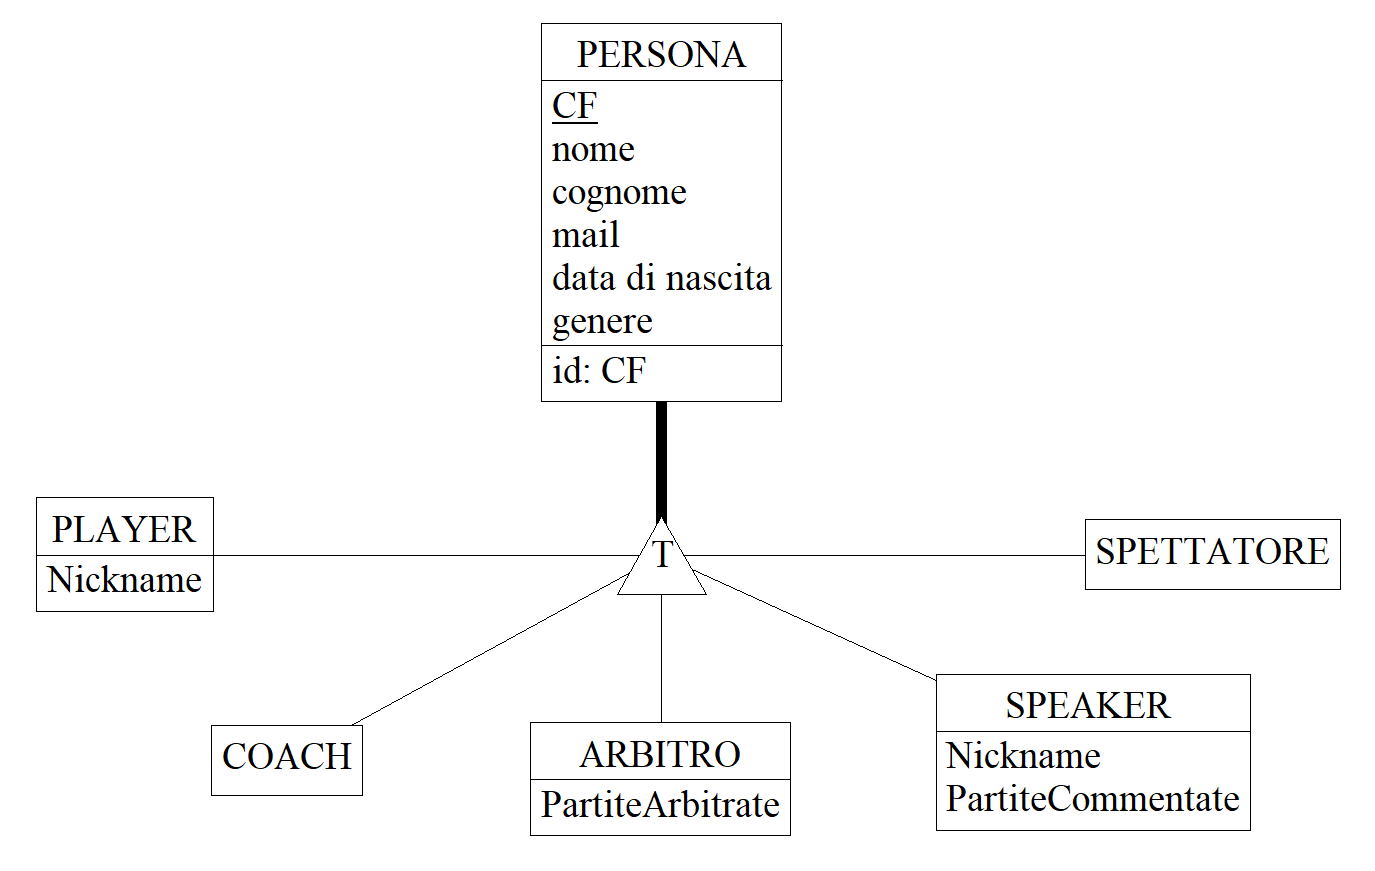
\includegraphics[scale=0.5]{img/ER_Persona.png}}
	\caption{Schema ER che espone le principali caratteristiche delle Persone}
	\label{img:ER_Persona}
\end{figure}

\section{Anteprima sviluppo dei "Videogiochi"}
In questa sezione verrà modellato l'aspetto di \textbf{Videogioco}. 
Il \textbf{Videogioco} ha un Nome, dal quale viene identificato, e una data di creazione.
 Esiste una relazione con una \textbf{Azienda di Videogiochi} la quale può creare più Videogiochi.
 
 Ogni Videogioco ha la propria \textbf{Tipologia} , ad esempio Sparatutto o Giochi di Carte. 
 
 Abbiamo la necessità di salvarci ogni \textbf{Player} a quale e quanti Videogiochi \textbf{Gioca}, memorizzando nel frattempo le sue Partite Vinte e le Partite Giocate \textit{(\underline{Nota Bene} : questi due attributi si riferisco a statistiche personali relative all'avanzamento nel gioco, non sono collegate in nessun modo all'entità dell'E-R chiamata "Partita", quest'ultima si riferisce esclusivamente ad un match all'interno di un Torneo).}
\begin{figure}[!htb]
	\centerline{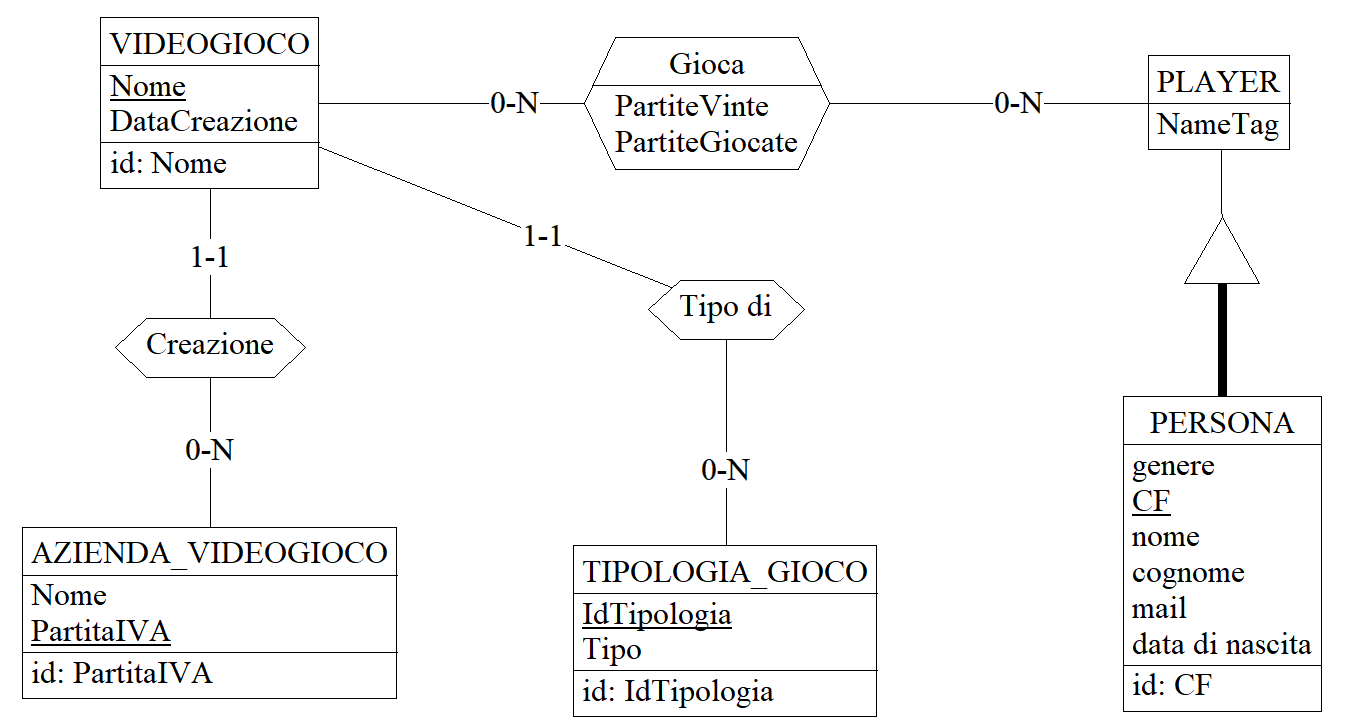
\includegraphics[scale=0.55]{img/ER_Videogiochi.png}}
	\caption{Schema ER che espone le principali caratteristiche dei Videogiochi}
	\label{img:ER_Videogiochi}
\end{figure}
\section{Anteprima sviluppo delle "Partite"}
In questa sezione verrà modellato l'aspetto di \textbf{Partita}.
L'entità \textbf{Partita} è probabilmente uno degli elementi più importanti e centrali di tutto lo schema E-R. Ogni \textbf{Partita} è identificata univocamente dalle due \textbf{Squadre} che parteciperanno all'incontro e dalla Data e Ora in cui si svolgerà.

Di ogni partita vogliamo memorizzarci ovviamente l'id delle due squadre che vi partecipano e anche l'id della \textbf{Squadra} che vincerà effettivamente lo scontro.

Ad ogni Partita inoltre partecipano due figure professionali, figlie della classe \textbf{Persona}: l'\textbf{Arbitro} che regolamenterà l'incontro e uno \textbf{Speaker} che lo commenterà.\\

Inoltre ogni \textbf{Partita} potrà avere degli Spettatori previo acquisto di un \textbf{Biglietto}. L'entità \textbf{Biglietto} è un template generale che associa ad una \textbf{Partita} un costo; lo \textbf{Spettatore} invece comprerà un biglietto effettivamente acquistabile, ovvero \textbf{AcquistoBiglietto}, che associa un \textbf{Biglietto} ad un unico \textbf{Spettatore}.
\begin{figure}[!htb]
	\centerline{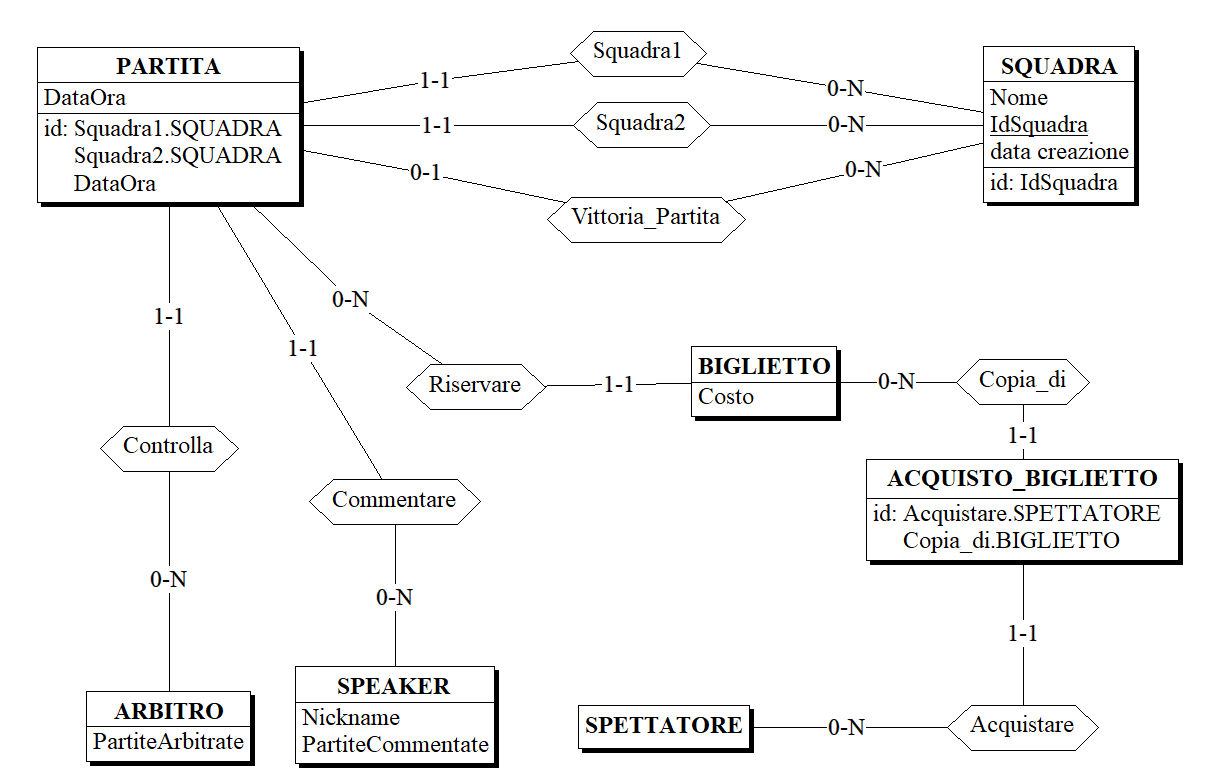
\includegraphics[scale=0.6]{img/ER_Partite.png}}
	\caption{Schema ER che espone le principali caratteristiche delle Partite}
	\label{img:ER_Partite}
\end{figure}
\section{Anteprima sviluppo dei "Tornei"}
In questa sezione verrà modellato l'aspetto di \textbf{Torneo}.
L'entità \textbf{Torneo} è il fulcro di tutto il nostro sistema informativo. Tutte le altre entità si collegano al Torneo in modo diretto o indiretto. 

Ogni \textbf{Torneo} è identificato da un numero progressivo e si vuole memorizzare: Data di inizio, Data di fine e il numero massimo di squadre che si possono iscrivere al torneo; vogliamo anche sapere su che \textbf{Videogioco} si baserà il Torneo (l'interno \textbf{Torneo} si baserà interamente su un unico Videogioco).

Ogni \textbf{Torneo} si svolge in una \textbf{Arena} situata in una città e può prevedere il finanziamento da parte di una \textbf{Sponsor}.

Ad ogni \textbf{Torneo} possono iscriversi più \textbf{Squadre} e si vuole memorizzare in particolare quale tra le due vincerà.

\begin{figure}[!htb]
	\centerline{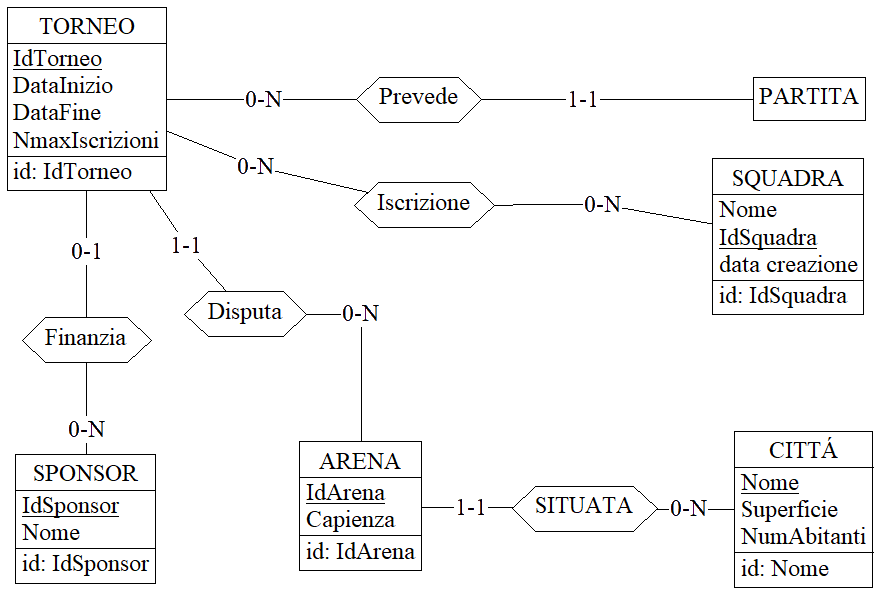
\includegraphics[scale=0.6]{img/ER_Tornei.png}}
	\caption{Schema ER che espone le principali caratteristiche dei Tornei}
	\label{img:ER_Tornei}
\end{figure}
\section{Schema Generale}
Di seguito verrà riportato lo schema concettuale generale, contenente tutte le entità e associazioni prima citate nelle varie sezioni superiori con l'aggiunta di entità secondarie di minor importanza.
\begin{figure}[!htb]
	\centerline{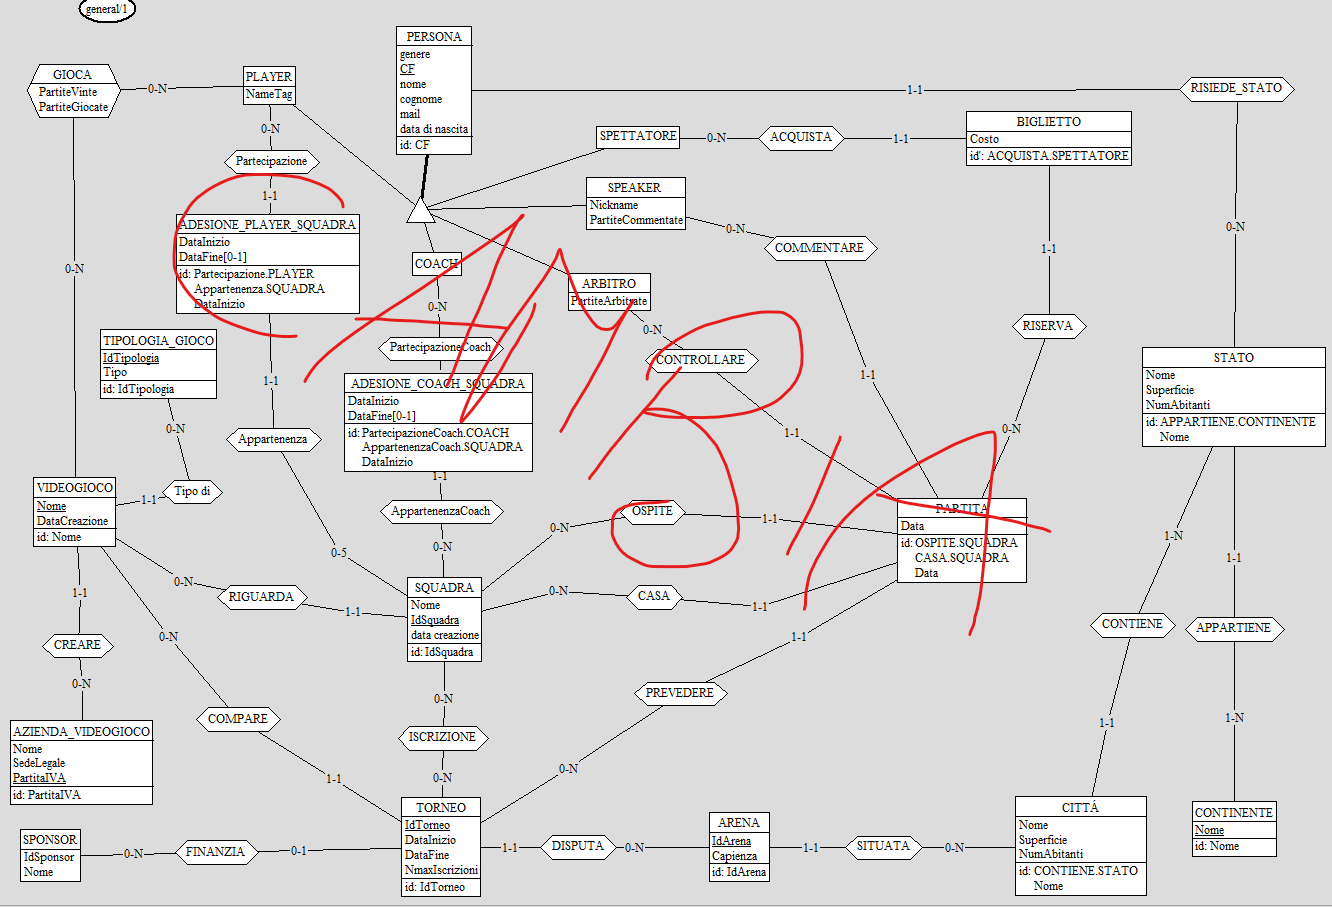
\includegraphics[scale=0.55]{img/ER_Generale.png}}
	\caption{Schema ER che espone lo schema concettuale finale}
	\label{img:ER_Generale}
\end{figure}

\chapter{Progettazione Logica}
\section{Stima del volume dei dati}
\renewcommand{\arraystretch}{1.5} %stretch scale delle celle
\setlength{\arrayrulewidth}{0.5mm}%grandezza bordi
\setlength{\tabcolsep}{10pt}%padding testo nelle celle
\setlength\doublerulesep{0.15cm}%spazio tra due linee

\begin{tabular}{|m{2cm}|c|m{2cm}|}
	\hline\rowcolor{pink}
	Soggetto & Tipo & Volume\\
	\hline\hline
	
	Player & E & 500.000\\
	\hline
	Videogiochi & E & 10\\
	\hline
	Tipologia Videogioco & E & 5\\
	\hline
	Gioca & A & 1.000.000\\
	\hline
	Azienda Videogioco & E & 5\\
	\hline
	 Squadra Riguarda Videogioco & A & 250.000\\
	
	\hline
	\hline
	
	Squadra & E & 100.000\\
	\hline
	Coach & E & 50.000\\
	\hline
	Adesione Player Squadra& E & 600.000\\ 
	\hline
	Adesione Coach Squadra& E & 75.000\\ 
	
	\hline
\end{tabular}
\setlength\doublerulesep{0.28cm} %spazio tra due linee
\begin{tabular}{|m{2cm}|c|m{2cm}|}
	\hline\rowcolor{pink}
	Soggetto & Tipo & Volume\\
	\hline\hline
	Speaker & E & 1.000\\
	\hline
	Arbitro & E & 1.000\\
	\hline
	Spettatori & E & 200.000.000\\
	\hline
	Acquisto Biglietto & E & 200.000.000\\ 
	\hline
	Sponsor & E & 35\\
	
	\hline\hline
	
	Tornei & E & 10.000\\
	\hline
	Partite & E & 450.000\\
	\hline
	Previste & A & 450.000\\ 
	\hline
	Iscrizioni Torneo & A & 100.000\\ 
	\hline
	
	\hline\hline
	
	Continente & E & 6\\
	\hline
	Stati & E & 30\\
	\hline
	Città & E & 60\\ 
	\hline
	Arene & E & 70\\ 
	\hline
	
	
\end{tabular}
\section{Descrizione delle operazioni principali e stima della loro frequenza}
Le operazioni da effettuare sono quelle già elencate nella fase di analisi. Segue una tabella
riportante la loro descrizione e relativa frequenza:
\begin{center}
	\begin{tabular}{|c|m{8cm}|c|}
		\hline\rowcolor{pink}
		Codice & Descrizione Operazione & Frequenza\\
		\hline\hline
		1 & Aggiunta di un nuovo Player & 50 al giorno\\ 
		\hline	
		2 & Aggiunta Videogioco giocato da un Player & 400 a settimana \\
		\hline
		3 & Aggiunta di un nuovo Spettatore & 30.000 a settimana \\
		\hline
		4 & Creazione di una Squadra & 100 al mese\\
		\hline 
		5 & Aggiunta di un Player ad una Squadra & 1.500 al mese\\ 
		\hline
		6 & Creazione di un Torneo & 1 a settimana\\ 
		\hline
		7 & Iscrizione di una Squadra ad un Torneo & 10 a settimana\\ 
		\hline
		8 & Creazione di nuove Partite in un Torneo & 45 a settimana\\ 
		\hline
		9 & Acquisto di un nuovo Biglietto & 30.000 a settimana\\ 
		\hline
		10 & Mostrare le squadre a cui partecipa un player & 30 a settimana\\
		\hline
	\end{tabular}
\end{center}
\section{Schemi di navigazione e tabelle degli accessi}
Sono riportate in seguito le tabelle degli accessi delle operazioni sopra riportate; inoltre, ove
non risulti banale, sono stati inseriti i relativi schemi di navigazione. Al fine del calcolo degli
costi, si considerano di peso doppio gli accessi in scrittura rispetto a quelli in lettura.
\renewcommand{\arraystretch}{1.15} %stretch scale delle celle
\setlength{\arrayrulewidth}{0.5mm}%grandezza bordi
\setlength{\tabcolsep}{10pt}%padding testo nelle celle
\setlength\doublerulesep{0.1cm}%spazio tra due linee
\subsection*{(1) Aggiunta di un nuovo Player}
Nell'entità Player viene aggiunta una tupla.
\begin{center}
	\begin{tabular}{|c|c|c|c|}
		\hline\rowcolor{pink}
		Concetto & Costrutto & Accessi & Tipo\\
		\hline\hline
		Player & E & 1 & S\\
		\hline\hline
		\multicolumn{2}{l}{
			\textbf{Totale:} 1S * 50 al giorno → 100 al giorno} \\
		\hline
	\end{tabular}
\end{center}
\subsection*{(2) Aggiunta di un videogioco giocato da un Player}
Presupponendo che sia Videogioco, sia Player siano già stati inseriti, è necessario semplicemente aggiungere una tupla alla tabella relativa all'associazione Gioca.
\begin{center}
	\begin{tabular}{|c|c|c|c|}
		\hline\rowcolor{pink}
		Concetto & Costrutto & Accessi & Tipo\\
		\hline\hline
		Gioca & A & 1 & S\\
		\hline\hline
		\multicolumn{2}{l}{%
			\textbf{Totale:} 1S * 400 a settimana → 800 a settimana} \\
		\hline
	\end{tabular}
\end{center}
\subsection*{(3) Aggiunta di un nuovo Spettatore}
Nell'entità spettatore viene aggiunta una tupla.
\begin{center}
	\begin{tabular}{|c|c|c|c|}
		\hline\rowcolor{pink}
		Concetto & Costrutto & Accessi & Tipo\\
		\hline\hline
		Spettatore & E & 1 & S\\
		\hline\hline
		\multicolumn{2}{l}{%
			\textbf{Totale:}  1S * 30.000 a settimana → 60.000 a settimana } \\
		\hline
	\end{tabular}
\end{center}
\subsection*{(4) Creazione di una Squadra}
Viene aggiunta una tupla all'entità Squadra, inoltre automaticamente, il player che ha creato la squadra viene iscritto, dunque viene scritta una tupla anche nell'associazione Adesione\_Player\_Squadra.
\begin{center}
	\begin{tabular}{|c|c|c|c|}
		\hline\rowcolor{pink}
		Concetto & Costrutto & Accessi & Tipo\\
		\hline
		Squadra & E & 1 & S\\
		\hline
		Adesione\_Player\_Squadra & A & 1 & S\\
		\hline\hline
		\multicolumn{2}{l}{%
			\textbf{Totale:} (1S + 1S) * 100 al mese  → 400 al mese} \\
		\hline\hline
	\end{tabular}
\end{center}
\subsection*{(5) Aggiunta di un Player ad una Squadra}
Inizialmente devo controllare che la squadra non sia completa, avendo una squadra da 1 a 5 membri, in media verranno fatte 3 letture, successivamente, se la squadra non è piena, viene aggiunta una tupla all'associazione Adesione\_Plyer\_Squadra.
\begin{center}
	\begin{tabular}{|c|c|c|c|}
		\hline\rowcolor{pink}
		Concetto & Costrutto & Accessi & Tipo\\
		\hline\hline		
		Adesione\_Plyer\_Squadra & E & 3 & L\\
		Adesione\_Player\_Squadra & A & 1 & S\\
		\hline
		\hline
		\multicolumn{2}{l}{%
			\textbf{Totale:} (3L + 2S) * 150.000 al giorno → 1.050.000 al giorno} \\
		\hline
	\end{tabular}
\end{center}
\subsection*{(6) Creazione di un Torneo}
Viene aggiunta una tupla all'entità Torneo.
\begin{center}
	\begin{tabular}{|c|c|c|c|}
		\hline\rowcolor{pink}
		Concetto & Costrutto & Accessi & Tipo\\
		\hline\hline		
		Torneo & E & 1 & S\\
		\hline
		\hline
		\multicolumn{2}{l}{%
			\textbf{Totale:} (1S) → 2 alla settimana} \\
		\hline
	\end{tabular}
\end{center}
\subsection*{(7) Iscrizione di una Squadra ad un Torneo}
\begin{center}
	\begin{tabular}{|c|c|c|c|}
		\hline\rowcolor{pink}
		Concetto & Costrutto & Accessi & Tipo\\
		\hline\hline		
		Iscrizione Squadra & A & 1 & S\\
		\hline
		\hline
		\multicolumn{2}{l}{%
			\textbf{Totale:}  1S * 8 a settimana → 16 a settimana} \\
		\hline
	\end{tabular}
\end{center}
\subsection*{(8) Creazione di nuove Partite in un Torneo}
\begin{center}
	\begin{tabular}{|c|c|c|c|}
		\hline\rowcolor{pink}
		Concetto & Costrutto & Accessi & Tipo\\
		\hline\hline		
		Partita & E & 45 & S\\
		Partita Prevista & A & 45 & S\\
		\hline
		\hline
		\multicolumn{2}{l}{%
			\textbf{Totale:} (45S + 45S)  → 180 a settimana} \\
		\hline
	\end{tabular}
\end{center}
\subsection*{(9) Acquisto di un nuovo Biglietto}
devo leggere il costo
\begin{center}
	\begin{tabular}{|c|c|c|c|}
		\hline\rowcolor{pink}
		Concetto & Costrutto & Accessi & Tipo\\
		\hline\hline		
		Acquistare & A & 1 & S\\
		Biglietto & E & 1 & L\\
		\hline
		\hline
		\multicolumn{2}{l}{%
			\textbf{Totale:} 1L + 2S → 150.000} \\
		\hline
	\end{tabular}
\end{center}
\subsection*{(10) Mostrare le squadre a cui partecipa un player}
Avendo nella tabella dei volumi 500.000 player totali e 600.000 adesione\_player\_squadra, ogni player partecipa in media a 1,2 squadre
\begin{center}
	\begin{tabular}{|c|c|c|c|}
		\hline\rowcolor{pink}
		Concetto & Costrutto & Accessi & Tipo\\
		\hline\hline		
		Adesione\_Player\_Squadra & E & 1,2 & L\\
		\hline
		\hline
		\multicolumn{2}{l}{%
			\textbf{Totale:} 1,2L → 36/settimana} \\
		\hline
	\end{tabular}
\end{center}
\section{Raffinamento dello schema}
\subsection*{Eliminazione Gerarchie}
Eliminazione delle gerarchie
Per l’eliminazione della gerarchia persona si è scelto di adottare l’approccio del collasso verso
il basso, replicando così gli attributi della Persona nelle seguenti entità: Player, Coach, Arbitro, Spettatore. 
Si è adottata questa strategia in
quanto si deve interagire con i clienti molto più spesso che con gli istruttori, e non si ha la
necessità che l’identificatore per tali entità sia globalmente univoco.
\subsection*{Scelta delle Chiavi}
Sin dall'inizio abbiamo scelto accuratamente tutte le chiavi per ogni entità; queste sono evidenziate senza ambiguità nello schema E-R.
\section{Analisi delle ridondanze}
\subsection*{Senza Ridondanza}
senza la ridondanza sul numero di biglietti venduti, leggo il costo del biglietto; in media ho 500 letture su acquisto-biglietto per vedere quanti sono stati venduti; ho una lettura su arena per verificarne la capienza.
\begin{center}
	\begin{tabular}{|c|c|c|c|}
		\hline\rowcolor{pink}
		Concetto & Costrutto & Accessi & Tipo\\
		\hline\hline		
		Acquistare & A & 1 & S\\
		Biglietto & E & 1 & L\\
		AcquistoBiglietto & E & 500 & L\\
		Arena & E & 1 & L\\
		\hline
		\hline
		\multicolumn{2}{l}{%
			\textbf{Totale:} (502L + 2S) * 30.000 → 15.180.000 ogni settimana} \\
		\hline
	\end{tabular}
\end{center}
\subsection*{Con la Ridondanza}
\begin{center}
	\begin{tabular}{|c|c|c|c|}
		\hline\rowcolor{pink}
		Concetto & Costrutto & Accessi & Tipo\\
		\hline\hline		
		Acquistare & A & 1 & S\\
		Biglietto & E & 1 & L\\		
		\hline
		\hline
		\multicolumn{2}{l}{%
			\textbf{Totale:} 1L + 2S → 150.000 ogni settimana} \\
		\hline
	\end{tabular}
\end{center}
\section{Traduzione di entità e associazioni in relazioni}

ACQUISTO\_BIGLIETTO((\underline{IdArena}, \underline{IdSquadra1}, \underline{IdSquadra2}, \underline{DataOra}) : BIGLIETTO, \underline{CF\_Spettatore}) \\

\noindent ADESIONE\_COACH\_SQUADRA(\underline{IdSquadra}: SQUADRA, \underline{CF\_Coach} : COACH, \underline{DataInizio}, DataFine*) \\

\noindent ADESIONE\_PLAYER\_SQUADRA(\underline{IdSquadra}: SQUADRA, \underline{CF\_Player}: PLAYER, \underline{DataInizio}, DataFine*) \\

\noindent ARBITRO(\underline{CF}, nome, cognome, genere, mail data\_di\_nascita, PartiteArbitrate) \\

\noindent ARENA(\underline{IdArena}, NomeArena, Capienza, (NomeStato, NomeCitta): CITTÀ) \\

\noindent AZIENDA\_VIDEOGIOCO(nome, \underline{partitaIVA}) \\

\noindent BIGLIETTO(\underline{IdArena} : ARENA, (\underline{IdSquadra1}, \underline{IdSquadra2}, \underline{DataOra}) : PARTITA, Costo) \\

\noindent CITTÀ(\underline{NomeStato}: STATO, \underline{Nome}, Superficie, NumAbitanti) \\

\noindent COACH(\underline{CF}, nome, cognome, genere, mail, data\_di\_nascita) \\

\noindent CONTINENTE(\underline{Nome}) \\

\noindent GIOCA(\underline{NomeVideogioco} : VIDEOGIOCO, \underline{CF\_Player} : PLAYER, PartiteVinte, PartiteGiocate) \\

\noindent ISCRIZIONE(\underline{IdTorneo} : TORNEO, \underline{IdSquadra} : SQUADRA) \\

\noindent PARTITA((\underline{IdSquadra2}, \underline{IdSquadra1}) : SQUADRA, \underline{DataOra}, CF\_Arbitro : ARBITRO, CF\_Speaker : SPEAKER, IdSquadraVincitrice* : SQUADRA, IdTorneo : TORNEO) \\

\noindent PLAYER(\underline{CF}, nome, cognome, genere, mail, data\_di\_nascita, Nickname, Nome\_Stato: STATO) \\

\noindent RIGUARDA(\underline{IdSquadra} : SQUADRA, \underline{NomeVideogioco} : VIDEOGIOCO) \\

\noindent SPEAKER(\underline{CF}, nome, cognome, genere, mail, data\_di\_nascita, Nickname, PartiteCommentate) \\

\noindent SPETTATORE(\underline{CF}, nome, cognome, genere, mail, data\_di\_nascita) \\

\noindent SPONSOR(\underline{IdSponsor}, Nome) \\

\noindent SQUADRA(nome, \underline{IdSquadra}, data\_creazione) \\

\noindent STATO(\underline{Nome}, Superficie, NumAbitanti, NomeContinente : CONTINENTE) \\

\noindent TIPOLOGIA\_GIOCO(\underline{IdTipologia}, Tipo) \\

\noindent TORNEO(\underline{IdTorneo}, DataInizio, DataFine*, NMaxIscrizioni, IdSponsor* : SPONSOR, NomeVideoGioco : VIDEOGIOCO, IdArena : ARENA, IdSquadraVincitrice* : SQUADRA) \\

\noindent VIDEOGIOCO(\underline{Nome}, DataCreazione, TipologiaGioco : TIPOLOGIA\_GIOCO, PartitaIVAAzienda : AZIENDA\_VIDEOGIOCO) \\







\section{Schema relazionale finale}


\chapter{Progettazione Fisica}
\section{Traduzione in SQL}
\subsection*{(1) Aggiunta di un nuovo Player}
\textcolor{blue}{INSERT INTO} player (CF, nome, cognomi, genere, mail, data\_di\_nascita, Nickname, Nome\_Stato)
\textcolor{blue}{VALUES} (?,?,?,?,?,?,?,?);

\subsection*{(2) Aggiunta di un videogioco giocato da un Player}
\textcolor{blue}{INSERT INTO} gioca(NomeVideogioco, CF\_Player, PartiteVinte, PartiteGiocate)
\textcolor{blue}{VALUES} (?,?,?,?);

\subsection*{(3) Aggiunta di un nuovo Spettatore}
\textcolor{blue}{INSERT INTO} spettatore(CF, nome, cognomi, genere, mail, data\_di\_nascita)
\textcolor{blue}{VALUES} (?,?,?,?,?,?);

\subsection*{(4) Creazione di una Squadra}
\textcolor{blue}{INSERT INTO} squadra(Nome, IdSquadra, data\_creazione)
\textcolor{blue}{VALUES} (?,IdSquadra,?);

\subsection*{(5) Aggiunta di un Player ad una Squadra}
\textcolor{blue}{INSERT INTO} adesione\_player\_squadra(IdSquadra, CF\_Player, DataInizio, DataFine)
\textcolor{blue}{VALUES} (?,?,?,null);

\subsection*{(6) Creazione di un Torneo}
\textcolor{blue}{INSERT INTO} torneo(IdTorneo, DataInizio, DataFine, NmaxIscrizioni, IdSponsor, NomeVideogioco,IdArena,IdSquadraVincitrice)
\textcolor{blue}{VALUES} (IdTorneo,?,?,?,?,?,?,?);

\subsection*{(7) Iscrizione di una Squadra ad un Torneo}
\textcolor{blue}{INSERT INTO} iscrizione(IdTorneo, IdSquadra)
\textcolor{blue}{VALUES} (?,?);

\subsection*{(8) Creazione di nuove Partite in un Torneo}
\textcolor{blue}{INSERT INTO} partita(IdSquadra1, IdSquadra2, DataOra, CF\_Arbitro,CF\_Speaker, IdSquadraVincitrice, IdTorneo)
\textcolor{blue}{VALUES} (?,?,?,?,?,?,?);

\subsection*{(9) Acquisto di un nuovo Biglietto}
\textcolor{blue}{INSERT INTO} acquisto\_biglietto(IdArena, IdSquadra1, IdSquadra2, DataOra, CF\_Spettatore)
\textcolor{blue}{VALUES} (?,?,?,?,?);

\chapter{Progettazione dell'Applicazione}
\section{Descrizione della scelta del linguaggio e del DBMS}
\section{Descrizione dell'architettura}
\section{Interfaccia Utente}
\subsection{Amministratore Torneo}
\subsection{Giocatore}
\end{document}
